% !TEX program = xelatex
% ¡Recuerda compilar con XeLaTeX o LuaLaTeX!
\documentclass{article}

% --- Cargar nuestro fichero de estilo ---
% Se asume que paper_style.sty está disponible o se usan paquetes estándar.
\usepackage{paper_style}

% --- PAQUETES PARA EL CONTENIDO DEL DOCUMENTO ---
\usepackage{graphicx}
\usepackage{subcaption}
\usepackage{amsmath}
\usepackage{booktabs}
\usepackage{geometry}
\usepackage{hyperref}
\usepackage{enumitem}
\usepackage{float}


% --- Cambiar numeración de subsecciones ---
\renewcommand{\thesubsection}{\alph{subsection})}
\renewcommand{\thesubsubsection}{$\bullet$}


% --- Información del Paper ---
\title{Seminario 1: \\ Aplicación web Futbol11.com estudio de usabilidad }
\author{
	Alejandro Martínez Riquelme \\
	Jordi Blasco Lozano \\
	\small Interacción Persona Máquina \\
	\small Universidad de Alicante
}
\date{\today}

% --- Comienzo del Documento ---
\begin{document}
	
	\maketitle

	\begin{abstract}
	\noindent 
	La página web \textbf{futbol11.com} es una plataforma de juegos de fútbol diarios que ha ganado gran popularidad con 9.17M de visitas mensuales. Sin embargo, el análisis de usabilidad mediante las heurísticas de Nielsen y la evaluación de accesibilidad según los criterios WCAG 2.2 revelan múltiples problemas críticos que afectan significativamente la experiencia del usuario, especialmente para personas con discapacidades.
	\end{abstract}

	
	\tableofcontents
	\newpage

	\section{Tecnicas de evaluación}
	
	\subsection{Evaluación Heurística}
	\noindent
	Hemos aplicado las \textbf{10 heurísticas de usabilidad de Jakob Nielsen} para identificar problemas de diseño de interacción, clasificando cada problema según su severidad (Leve, Media, Grave).

	\subsection{Evaluación de Accesibilidad}
	\noindent
	Utilizamos múltiples enfoques para evaluar el cumplimiento de las \textbf{Web Content Accessibility Guidelines (WCAG) 2.2}:
	\begin{enumerate}
		\item \textbf{Evaluación automática y manual}: Revisión de criterios específicos utilizando herramientas especializadas y valoración humana.
		\item \textbf{Evaluación con lectores de pantalla}: Simulación de uso real.
	\end{enumerate}

	\section{Análisis de Problemas de Usabilidad}

	\subsection{Visibilidad del Estado del Sistema}
	\noindent
	\textbf{Problema Detectado}: Ausencia de retroalimentación clara durante el proceso de juego.
	
	\noindent
	\textbf{Ejemplo Concreto}: Durante los juegos cronometrados, el usuario no recibe indicaciones claras sobre el estado de su progreso, tiempo restante o puntuación actual hasta completar la tarea.
	
	\noindent
	\textbf{Severidad}: Media
	
	\noindent
	\textbf{Propuesta de Mejora}: Implementar indicadores visuales persistentes que muestren el progreso en tiempo real, incluyendo barras de progreso, contadores de tiempo visibles y retroalimentación inmediata para cada acción del usuario.

	\subsection{Relación entre Sistema y Mundo Real}
	\noindent
	\textbf{Problema Detectado}: Uso de terminología específica del juego sin explicación.
	
	\noindent
	\textbf{Ejemplo Concreto}: Términos como ``futbol11 connections'' o ``futbol top10'' aparecen sin contexto explicativo para usuarios nuevos, dificultando la comprensión inmediata de la funcionalidad.
	
	\noindent
	\textbf{Severidad}: Leve
	
	\noindent
	\textbf{Propuesta de Mejora}: Incluir tooltips explicativos o una guía introductoria que explique la terminología específica del sitio utilizando lenguaje familiar para el usuario promedio.

	\subsection{Control y Libertad del Usuario}
	\noindent
	\textbf{Problema Detectado}: Limitada capacidad de deshacer acciones en juegos cronometrados.
	
	\noindent
	\textbf{Ejemplo Concreto}: Una vez iniciado un juego con tiempo límite, el usuario no puede pausar, reiniciar o salir sin perder todo el progreso, lo que genera frustración especialmente en dispositivos móviles donde pueden ocurrir interrupciones.
	
	\noindent
	\textbf{Severidad}: Grave
	
	\noindent
	\textbf{Propuesta de Mejora}: Implementar funciones de pausa, opciones de guardar progreso y confirmaciones antes de salir de juegos en curso. Permitir al usuario retomar juegos interrumpidos.

	\subsection{Consistencia y Estándares}
	\noindent
	\textbf{Problema Detectado}: Inconsistencia en la interfaz entre diferentes tipos de juegos.
	
	\noindent
	\textbf{Ejemplo Concreto}: Los diferentes juegos (Futbol11, Connections, Top10) presentan diseños de interface distintos, patrones de navegación inconsistentes y diferentes ubicaciones para elementos similares.
	
	\noindent
	\textbf{Severidad}: Leve
	
	\noindent
	\textbf{Propuesta de Mejora}: Crear un sistema de diseño unificado con componentes reutilizables, patrones de navegación estándar y una identidad visual coherente en todos los juegos.

	\subsection{Prevención de Errores}
	\noindent
	\textbf{Problema Detectado}: Falta de validación preventiva en los campos de entrada.
	
	\noindent
	\textbf{Ejemplo Concreto}: Al introducir nombres de jugadores, el sistema no ofrece sugerencias automáticas ni previene errores ortográficos comunes, lo que resulta en respuestas incorrectas por problemas de escritura más que de conocimiento.
	
	\noindent
	\textbf{Severidad}: Media
	
	\noindent
	\textbf{Propuesta de Mejora}: Implementar autocompletado inteligente, corrección ortográfica automática y sugerencias contextuales basadas en la entrada parcial del usuario.

	\subsection{Reconocer en Lugar de Recordar}
	\noindent
	\textbf{Problema Detectado}: Dependencia excesiva de la memoria del usuario para nombres exactos.
	
	\noindent
	\textbf{Ejemplo Concreto}: Los usuarios deben recordar y escribir nombres completos exactos de jugadores sin ayuda visual o sugerencias, lo que dificulta especialmente nombres con caracteres especiales o acentos.
	
	\noindent
	\textbf{Severidad}: Media
	
	\noindent
	\textbf{Propuesta de Mejora}: Integrar un sistema de sugerencias visuales, mostrar fotografías de jugadores como pistas adicionales y permitir búsquedas aproximadas.

	\subsection{Flexibilidad y Eficiencia de Uso}
	\noindent
	\textbf{Problema Detectado}: Ausencia de opciones de personalización para usuarios experimentados.
	
	\noindent
	\textbf{Ejemplo Concreto}: No existen atajos de teclado, configuraciones de dificultad personalizables o modos acelerados para usuarios que dominan los juegos básicos.
	
	\noindent
	\textbf{Severidad}: Media
	
	\noindent
	\textbf{Propuesta de Mejora}: Implementar niveles de dificultad configurables, atajos de teclado, y modos de juego avanzados que permitan a usuarios experimentados optimizar su experiencia.

	\subsection{Estética y Diseño Minimalista}
	\noindent
	\textbf{Problema Detectado}: Sobrecarga visual y elementos distractores.
	
	\noindent
	\textbf{Ejemplo Concreto}: La presencia de múltiples anuncios, elementos decorativos innecesarios y una densidad de información excesiva interfiere con la concentración requerida para los juegos cronometrados.
	
	\noindent
	\textbf{Severidad}: Grave
	
	\noindent
	\textbf{Propuesta de Mejora}: Simplificar la interfaz eliminando elementos no esenciales, optimizar la colocación de anuncios y crear espacios de respiro visual que mejoren la concentración del usuario.

	\subsection{Ayuda para Reconocer y Recuperarse de Errores}
	\noindent
	\textbf{Problema Detectado}: Mensajes de error poco informativos.
	
	\noindent
	\textbf{Ejemplo Concreto}: Cuando un usuario introduce una respuesta incorrecta, el sistema simplemente la marca como errónea sin proporcionar pistas sobre por qué falló o cómo corregirla.
	
	\noindent
	\textbf{Severidad}: Media
	
	\noindent
	\textbf{Propuesta de Mejora}: Diseñar mensajes de error constructivos que expliquen específicamente qué salió mal y ofrezcan sugerencias para la corrección, incluyendo alternativas válidas cuando sea apropiado.

	\subsection{Ayuda y Documentación}
	\noindent
	\textbf{Problema Detectado}: Ausencia de documentación centralizada y ayuda contextual.
	
	\noindent
	\textbf{Ejemplo Concreto}: Los usuarios nuevos deben descifrar las reglas de cada juego por ensayo y error, sin acceso a tutoriales interactivos, FAQ o guías de usuario.
	
	\noindent
	\textbf{Severidad}: Media
	
	\noindent
	\textbf{Propuesta de Mejora}: Crear una sección de ayuda comprensiva con tutoriales interactivos, videos explicativos y una base de conocimientos searchable que cubra todos los aspectos de la plataforma.

	\section{Análisis de Problemas de Accesibilidad}

	\noindent
	Hemos utilizado Skynet para hacer el analisis atomatico de la accesibilidad sobre la web, hemos obtenido un score de 0\% con 71 fallos según WCAG 2.2 los cuales los describiremos acontinuación. También se explicarán los criterios utilizados personalmente mediante herramientas de valoración manual como 'Accessibility Insights' para la valoración del criterio 3.2.2 entre otros.

	\begin{figure}[H]
	\centering
	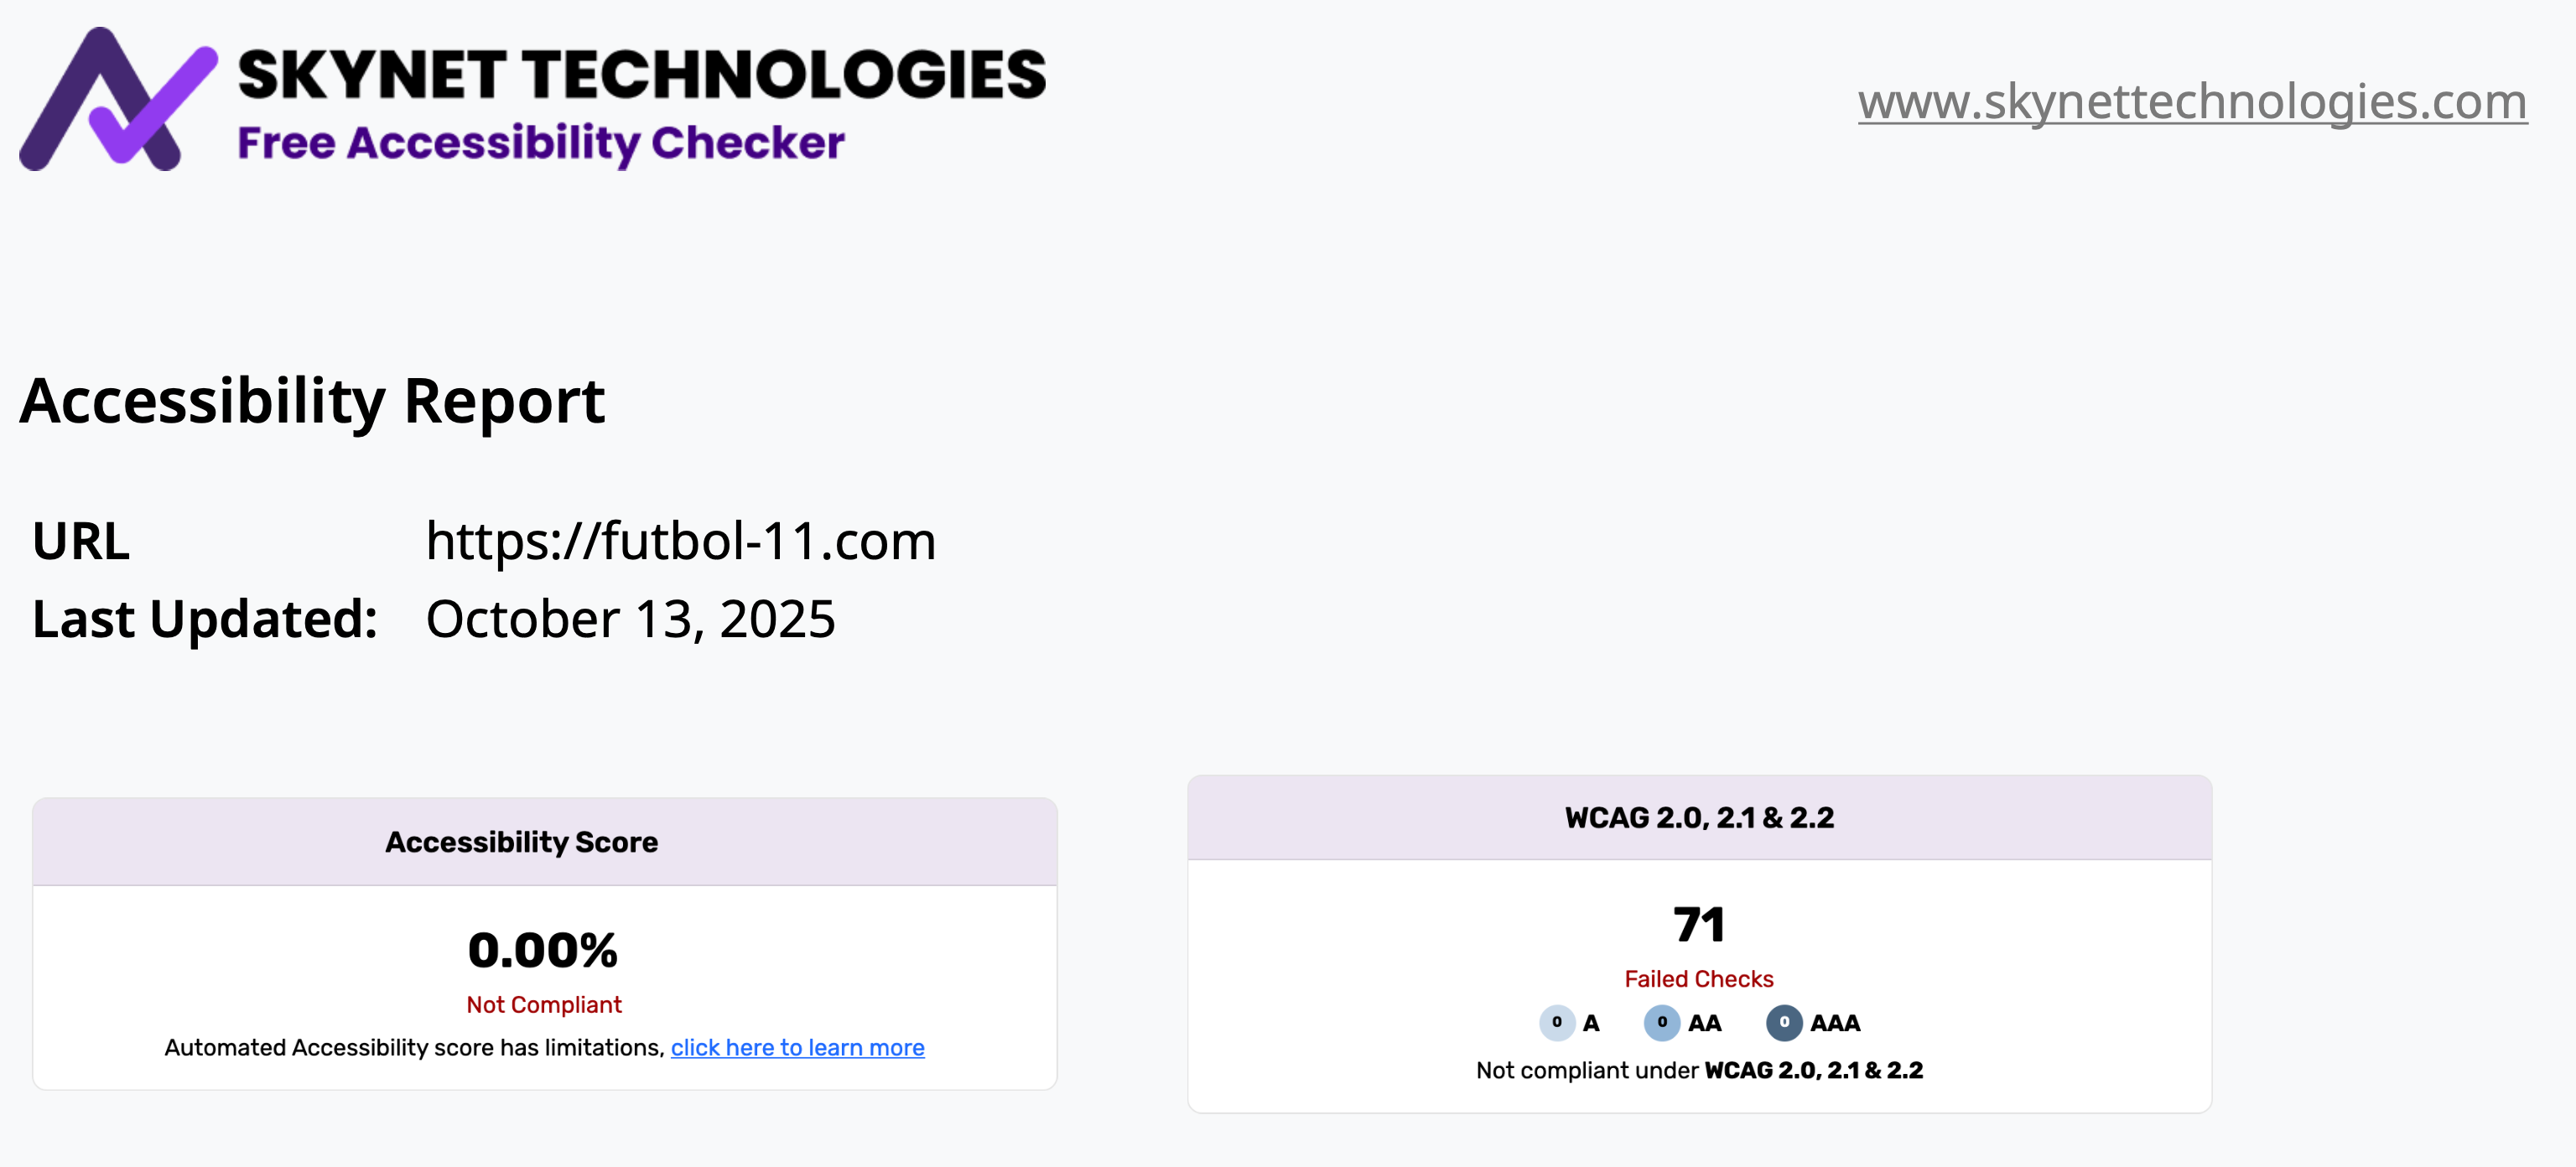
\includegraphics[width=\textwidth]{skynet.png}
	\caption{Análisis de skynet}
	\end{figure}


	\subsection{Evaluación según WCAG 2.2}

	\vspace{0.3cm}
	\noindent
	$\bullet$ \textbf{Principio 1: Perceptible}
	\vspace{0.3cm}
	
	\noindent
	\textbf{Criterio 1.1.1 - Contenido no textual}
	
	\noindent
	\textbf{Problema}: Las imágenes de jugadores y equipos carecen de texto alternativo descriptivo.
	
	\noindent
	\textbf{Severidad}: Grave
	
	\noindent
	\textbf{Impacto}: Los usuarios de lectores de pantalla no pueden identificar el contenido visual esencial para completar los juegos.
	
	\noindent
	\textbf{Recomendación}: Implementar texto alternativo descriptivo para todas las imágenes, especificando nombres de jugadores, equipos y contexto relevante.
	
	\vspace{0.5cm}
	
	\noindent
	\textbf{Criterio 1.4.3 - Contraste mínimo}
	
	\noindent
	\textbf{Problema}: Múltiples elementos presentan contraste insuficiente entre texto y fondo, especialmente en botones de acción y campos de entrada.
	
	\noindent
	\textbf{Severidad}: Media
	
	\noindent
	\textbf{Impacto}: Usuarios con baja visión o daltonismo tienen dificultades para distinguir elementos interactivos.
	
	\noindent
	\textbf{Recomendación}: Ajustar los contrastes para cumplir con la ratio mínima de 4.5:1 para texto normal y 3:1 para texto grande.

	\vspace{0.3cm}
	\noindent
	$\bullet$ \textbf{Principio 2: Operable}
	\vspace{0.3cm}
	
	\noindent
	\textbf{Criterio 2.1.1 - Teclado}
	
	\noindent
	\textbf{Problema}: Algunos elementos interactivos no son accesibles mediante navegación por teclado, especialmente en juegos cronometrados.
	
	\noindent
	\textbf{Severidad}: Grave
	
	\noindent
	\textbf{Impacto}: Usuarios que dependen de navegación por teclado no pueden completar los juegos.
	
	\noindent
	\textbf{Recomendación}: Asegurar que todos los elementos interactivos sean accesibles mediante teclado con un orden de tabulación lógico.
	
	\vspace{0.5cm}
	
	\noindent
	\textbf{Criterio 2.4.3 - Orden del foco}
	
	\noindent
	\textbf{Problema}: El orden de navegación por teclado no sigue una secuencia lógica, saltando entre elementos de manera impredecible.
	
	\noindent
	\textbf{Severidad}: Media
	
	\noindent
	\textbf{Impacto}: Confusión y pérdida de orientación para usuarios de tecnologías asistivas.
	
	\noindent
	\textbf{Recomendación}: Establecer un orden de tabulación coherente que siga el flujo visual esperado de la página.

	\vspace{0.3cm}
	\noindent
	$\bullet$ \textbf{Principio 3: Comprensible}
	\vspace{0.3cm}
	
	\noindent
	\textbf{Criterio 3.2.2 - Al recibir el foco}
	
	\noindent
	\textbf{Problema}: La publicidad al recibir el foco cambia de contenido inesperadamente, especialmente en dispositivos móviles.
	
	\noindent
	\textbf{Severidad}: Media
	
	\noindent
	\textbf{Impacto}: Desorientación y pérdida de control para usuarios de tecnologías asistivas.
	
	\noindent
	\textbf{Recomendación}: Eliminar cambios automáticos al recibir el foco, requiriendo acción explícita del usuario.
	
	\vspace{0.5cm}
	
	\noindent
	\textbf{Criterio 3.3.2 - Etiquetas o instrucciones}
	
	\noindent
	\textbf{Problema}: Campos de entrada carecen de etiquetas claras y instrucciones específicas sobre el formato esperado.
	
	\noindent
	\textbf{Severidad}: Grave
	
	\noindent
	\textbf{Impacto}: Usuarios con discapacidades cognitivas no comprenden qué información se solicita.
	
	\noindent
	\textbf{Recomendación}: Proporcionar etiquetas claras, placeholder text descriptivo e instrucciones específicas para cada campo.

	\vspace{0.3cm}
	\noindent
	$\bullet$ \textbf{Principio 4: Robusto}
	\vspace{0.3cm}
	
	\noindent
	\textbf{Criterio 4.1.2 - Nombre, función, valor}
	
	\noindent
	\textbf{Problema}: Elementos personalizados no exponen correctamente su función y estado a las tecnologías asistivas.
	
	\noindent
	\textbf{Severidad}: Grave
	\noindent
	\textbf{Impacto}: Lectores de pantalla no pueden comunicar efectivamente la funcionalidad de elementos críticos.
	
	\noindent
	\textbf{Recomendación}: Implementar atributos ARIA apropiados y asegurar que todos los elementos personalizados sean interpretables por tecnologías asistivas.

	\section{Evaluación con Lectores de Pantalla}
	\noindent Hemos elegido una aplicación de juegos la cual los lectores de pantalla no son aplicables en algunos juegos que requieren de prestar atencion visual, pero la mayoria de juegos podrian perfectamente presentar información en formato audio como cuando hay equipos, banderas, etc... Todos estos elementos podrían ser perfectamente accesibles pero como veremos acontinuación no lo son.
	
	

	\subsection{Experiencia con el Narrador de Windows}
	
	\noindent
	\textbf{Problemas Identificados}:
	\begin{enumerate}
		\item \textbf{Navegación de juegos}: Los lectores de pantalla no pueden interpretar correctamente la estructura de los juegos, leyendo solo coordenadas vacías en lugar del contenido real.
		\item \textbf{Retroalimentación de acciones}: Cuando el usuario realiza una acción (introducir una respuesta), el lector no proporciona confirmación audible del resultado.
		\item \textbf{Elementos temporales}: Los cronómetros y contadores de tiempo no son anunciados por el lector de pantalla, dejando al usuario sin información crucial sobre el progreso del juego.
	\end{enumerate}

	\subsection{Experiencia con VoiceOver (macOS)}
	
	\noindent
	\textbf{Problemas Similares}:
	\begin{enumerate}
		\item \textbf{Etiquetas faltantes}: Muchos botones y enlaces carecen de etiquetas descriptivas apropiadas.
		\item \textbf{Navegación por landmarks}: La página no utiliza elementos semánticos HTML5 apropiados, dificultando la navegación rápida por secciones.
	\end{enumerate}

	
	\section{Propuestas de mejora}

	\subsection{Acciones Inmediatas (Alta Prioridad)}
	\noindent
	\begin{enumerate}
		\item Implementar texto alternativo para todas las imágenes y elementos visuales críticos para el funcionamiento de los juegos.
		\item Corregir problemas de teclado asegurando que todos los elementos interactivos sean accesibles mediante navegación por teclado.
		\item Añadir etiquetas ARIA apropiadas para elementos personalizados y dinámicos.
		\item Mejorar el contraste de colores para cumplir con estándares WCAG AA.
	\end{enumerate}

	\subsection{Acciones a Medio Plazo (Prioridad Media)}
	\noindent
	\begin{enumerate}
		\item Desarrollar modo de accesibilidad específico que simplifique la interfaz y proporcione alternativas textuales completas.
		\item Implementar sistema de ayuda contextual con tutoriales interactivos y documentación comprehensiva.
		\item Crear opciones de personalización para tiempo de juego, dificultad y método de entrada.
		\item Optimizar la experiencia móvil considerando las necesidades de accesibilidad específicas de dispositivos táctiles.
	\end{enumerate}

	\subsection{Acciones a Largo Plazo (Mejora Continua)}
	\noindent
	\begin{enumerate}
		\item Establecer programa de testing con usuarios reales incluyendo personas con diversas discapacidades.
		\item Implementar monitoreo automático de accesibilidad como parte del proceso de desarrollo.
		\item Crear versiones alternativas de juegos que no dependan exclusivamente de elementos visuales.
		\item Desarrollar API de accesibilidad para integraciones futuras con tecnologías asistivas avanzadas.
	\end{enumerate}
\newpage
	\section{Conclusiones}

	\noindent
	Futbol11.com presenta problemas significativos tanto en usabilidad como en accesibilidad que afectan negativamente la experiencia de una gran parte de sus 9.17M de usuarios mensuales. Los problemas identificados no solo limitan el acceso a usuarios con discapacidades, sino que también reducen la eficiencia y satisfacción de todos los usuarios. A lo largo de este análisis, se ha evidenciado que la aplicación de las heurísticas de Nielsen revela deficiencias en aspectos fundamentales como la visibilidad del estado del sistema, el control del usuario y la prevención de errores, lo que genera frustración y una curva de aprendizaje pronunciada para los visitantes frecuentes. \\

	\noindent
	En el ámbito de la accesibilidad, el cumplimiento parcial de los principios WCAG 2.2, particularmente en percepción, operabilidad y comprensión, subraya la necesidad de una revisión integral para garantizar la inclusión universal. Por ejemplo, la ausencia de texto alternativo en imágenes y el contraste insuficiente no solo excluyen a usuarios con discapacidades visuales, sino que también impactan en la legibilidad general de la interfaz bajo condiciones variables de iluminación o en dispositivos móviles. Las evaluaciones con lectores de pantalla como Narrador de Windows y VoiceOver confirman que la navegación y la retroalimentación sonora son inadecuadas, lo que impide una interacción fluida y equitativa para un público diverso. \\

	\noindent
	Las propuestas de mejora delineadas, desde acciones inmediatas como la implementación de ARIA y mejoras en el contraste hasta iniciativas a largo plazo como pruebas con usuarios reales, representan un camino viable hacia una plataforma más inclusiva y eficiente. Adoptar un enfoque centrado en el usuario no solo elevaría el cumplimiento normativo, sino que también potenciaría la retención de usuarios y la reputación de futbol11.com en un mercado competitivo de juegos en línea. En última instancia, este estudio resalta la importancia de integrar la usabilidad y accesibilidad desde las fases iniciales del diseño, alineándose con los estándares internacionales de interacción persona-máquina para fomentar experiencias digitales equitativas y satisfactorias.

\end{document}